\chapter{Kingdom of Fife}
{\entryfont \DndDropCapLine{F}or over a thousand years, the Kingdom of Fife stood as a beacon of strength and unity in the northern lands, founded by the legendary hero Dundax. From the city of Dundee, the royal bloodline ruled over a prosperous kingdom, its history intertwined with tales of valour, honour, and a long-forgotten prophecy that once foretold its fall. Now, on the eve of a grand wedding that promised to secure peace for generations, whispers of strange and unsettling phenomena began to emerge, though few took them seriously enough to cloud the celebrations.

}

\subsubsection*{The Birth of Dundax}
{\entryfont In the time before the founding of the grand city of Dundee, the lands of what would become the Kingdom of Fife were wild and untamed, roamed by warring clans and scattered settlements. It was during this era, in the year 20 B.D., that Dundax, the legendary hero, was born. Raised in the rugged hills of the north, Dundax was said to possess a strength and wisdom beyond his years, earning him the admiration of both chieftains and common folk alike. Tales of his feats spread quickly - how he single-handedly defended his village from raiders, how he tamed the wild beasts of the forests, and how he united rival clans through his courage and diplomacy.

Yet, it wasn't just his physical might that made Dundax a hero in the eyes of the people. A dreamer and a visionary, Dundax saw a future for Fife that transcended the tribal skirmishes of his time. He imagined a kingdom, one where peace could flourish and where his people could thrive under a united banner.}

\subsubsection*{The Founding of Dundee}
{\entryfont By the year 0 A.D., Dundax had grown into a man of great renown. It was in this year that he gathered his followers and founded the city of Dundee. From the city's grand walls, rising from the banks of the silvery Tay River, Dundax proclaimed the birth of the Kingdom of Fife - a land where unity and prosperity would reign.

Dundee itself was a marvel of its time. Surrounded by fertile lands and guarded by the natural barrier of the river, it became a beacon for traders and settlers from across the land. Under the wise rule of Dundax, the kingdom began to grow, with smaller settlements and clans swearing fealty to this new vision of peace and unity.

However, as Dundax stood on the heights of his newly founded city, a shadow loomed. Malyroth, a farseer from Anstruther, approached the city and spoke a prophecy that would echo through the ages: \textbf{"The prophecy is written. Dundee will fall!"} The words, though vague, struck fear into the hearts of those who heard them at the time. But as decades turned into centuries and the kingdom prospered without incident, the prophecy gradually faded into obscurity, remembered only by a select few scholars and keepers of ancient knowledge. For the vast majority of Fife's people, the prophecy of Dundee's fall became little more than an old myth, a forgotten relic of the past.}

\subsubsection*{The Founding of the Knights of Crail}
{\entryfont In the year 450 A.D., Prolon I, a visionary leader from Fyfdonia, a fertile region south of Dundee, founded the Order of the Knights of Crail. The knights quickly became known as a mystical and formidable force, renowned for their mastery of combat and their ability to ride giant, flying eagles. This gave them an unprecedented advantage in battle, and they earned a reputation as warriors who never opted out of a fight and were never defeated. The Knights of Crail became a symbol of Fyfdonia's strength and were revered not only for their prowess but for their mysterious and unwavering code of honor. Their presence in the region began to shape the political and military landscape of Fife.}

\subsubsection*{The Great Eagle War}
{\entryfont By the year 743 A.D., tensions between the principalities of Fyfdonia and Angus reached a breaking point, leading to the outbreak of the Great Eagle War. This conflict, named for the flying eagles of the Knights of Crail, saw Fyfdonia and Angus locked in bitter combat. Dundee, though officially neutral, was heavily affected by the conflict between its northern and southern neighbours.

The war raged for years, with both sides suffering significant losses. However, the might of the Knights of Crail, launching devastating aerial attacks from their eagles, proved overwhelming for Angus's ground forces. In a momentous agreement, the principalities of Angus and Fyfdonia were unified into a single kingdom, marking the birth of the Kingdom of Fife. The city of Dundee, with its strategic position and deep cultural significance, was declared the capital of this newly united realm. The Great Eagle War, though devastating, resulted in a lasting peace, with the once-warring regions now working together as a single kingdom.}

\subsubsection*{Angus McFife I and Iona McDougall}
{\entryfont In the year 992 A.D., a great celebration was planned in Dundee. \textbf{Angus McFife I}, Prince of Fife, was set to wed Iona McDougall, daughter of Ser Proletius, Grandmaster of the Knights of Crail. The marriage was not just a union of two noble houses, but a symbol of the continued unity and strength of the kingdom. It was said that the wedding would solidify the bond between the royal family and the Knights of Crail, ensuring peace and stability for generations to come.

The city of Dundee was alive with excitement. Streets were adorned with banners, musicians played in the marketplaces, and people from across the kingdom flocked to witness the royal wedding. Angus McFife I, a young man of great charm and valour, was beloved by the people. His bride-to-be, Iona, was known for her beauty and intellect, as well as her skill in diplomacy. Together, they seemed poised to usher the Kingdom of Fife into a new age of prosperity.

Yet, as the kingdom prepared for the joyous event, whispers began to surface of strange occurrences in the mountainous regions beyond the river Tay. There were scattered sightings of the kingdom's famed unicorns - creatures known for their}
\onecolumn
\begin{multicols}{2}
{\entryfont \noindent gentle nature and their gleaming, pure white coats - behaving in ways that unsettled those who saw them. Normally kind and serene, these unicorns were seen acting erratically - skittish and aggressive, fleeing from human contact. Stranger still were reports of unicorns with unusual, festering wounds that never seemed to heal, wounds that glowed with an eerie, unnatural light. Their once-brilliant fur had grown dull and dirty, as though corrupted by a dark and malevolent force.

The sightings, however, were few and far between, scattered across the remote and wild mountains where only the bravest of travellers ventured. As such, most dismissed these reports as exaggerations or simple superstitions. After all, the unicorns had always been a symbol of purity and light, cherished by the people of Fife for centuries. The odd behaviour of a few unicorns in distant lands seemed insignificant in the face of the grand wedding and the continued prosperity of the kingdom.

Still, for those who had encountered the strange unicorns first-hand, there was a growing sense of unease, though it remained unspoken. The royal family and the Knights of Crail quietly noted the reports but took no public action, choosing not to alarm the populace on the eve of such an important event.

The stage was set, not just for a royal wedding, but for a turning point in the history of Fife. As the city of Dundee prepared for joy, unseen forces began to stir in the shadows. And so, on the eve of Angus and Iona's wedding, the Kingdom of Fife stood on the precipice of its greatest trial. Would the kingdom survive the strange occurrences creeping from the mountains beyond the Tay, or was this the beginning of the end for the proud land that Dundax had founded so long ago? Only time would tell...}
\end{multicols}
\vspace*{-4em}\hfill\\
\phantomsection\addcontentsline{toc}{section}{Map of the Kingdom of Fife}
\noindent\begin{tikzpicture}[remember picture, overlay]%
		\node[opacity=1,inner sep=0pt,yshift=-3.35cm] at (current page.center){\includegraphics[width=\textwidth +8pt, keepaspectratio]{Kingdom_of_Fife_Map.png}};%
\end{tikzpicture}%
\twocolumn

\clearpage

\section*{Factions}\phantomsection\addcontentsline{toc}{section}{Factions}
\DndDropCapLine{C}{\entryfont aledonia is a realm of countless powers, where kingdoms, orders, and ancient enclaves shape the world through might, magic, and invention. From frostbound mountains to mist-shrouded isles, from hidden elven cities to roaring dwarven forges, each faction pursues its own vision of strength, honour, or dominion. Some clash in bitter rivalry, others form uneasy alliances - but all leave their mark on the ever-turning tale of Caledonia.}
\subsection*{Kingdom of Fife}
\vspace*{-0.3\fontdimen6\font}\hfill\\\begin{tabular}{p{0.3\textwidth}p{0.1325\textwidth}}
	\hspace*{-1.2em}\begin{tabular}[t]{p{0.325\textwidth}}
		{\entryfont The Kingdom of Fife, ruled by King Dundax \RoyalRoman{XIII} and his heir Prince Angus McFife, dominates eastern Caledonia from its thousand-year-old capital of Dundee - founded by the legendary hero Dundax himself. Here, noble warriors train beneath the ramparts of grand castles,\linebreak}
	\end{tabular}
	&
	\vspace*{-2.4em}\begin{tabular}[t]{p{0.1325\textwidth}}
		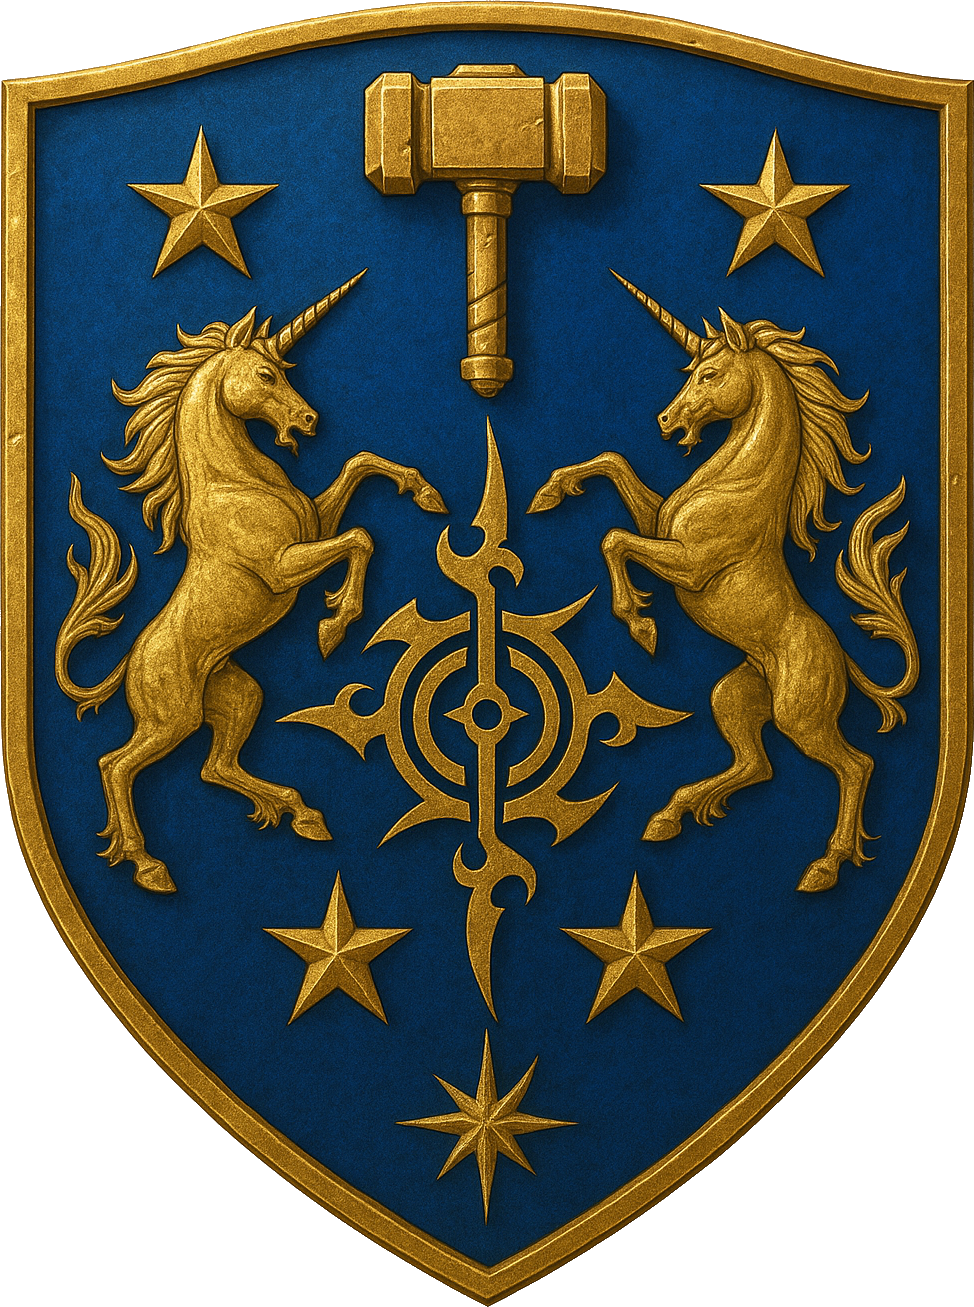
\includegraphics[width=0.1325\textwidth]{Factions/Kingdom_of_Fife.png}
	\end{tabular}
\end{tabular}
\vspace*{-1.65\fontdimen6\font}\hfill\\{\entryfont and centuries-old traditions guide every feast and festival. In the aftermath of the Great Eagle War, Fife's martial defences now rest almost entirely upon the Knights of Crail - those eagle-borne champions who alone bear the burden of war. Their soaring patrols and rapid response keep the kingdom's borders secure, freeing King Dundax \RoyalRoman{XIII} and Prince Angus McFife to govern in peace.}
\subsection*{Templar Knights of Crail}
\vspace*{-0.3\fontdimen6\font}\hfill\\\begin{tabular}{p{0.3\textwidth}p{0.1325\textwidth}}
	\hspace*{-1.2em}\begin{tabular}[t]{p{0.325\textwidth}}
		{\entryfont Founded in 450 AD by Prolon I, the Knights of Crail secured their edge by taming the Great Eagles of the nearby peaks, charging into battle on raptor-back with steel and talon alike. In 743 AD they waged a brutal war against Angus and Fyfdonia - eagle-borne lancers\linebreak}
	\end{tabular}
	&
	\vspace*{-2.4em}\begin{tabular}[t]{p{0.1325\textwidth}}
		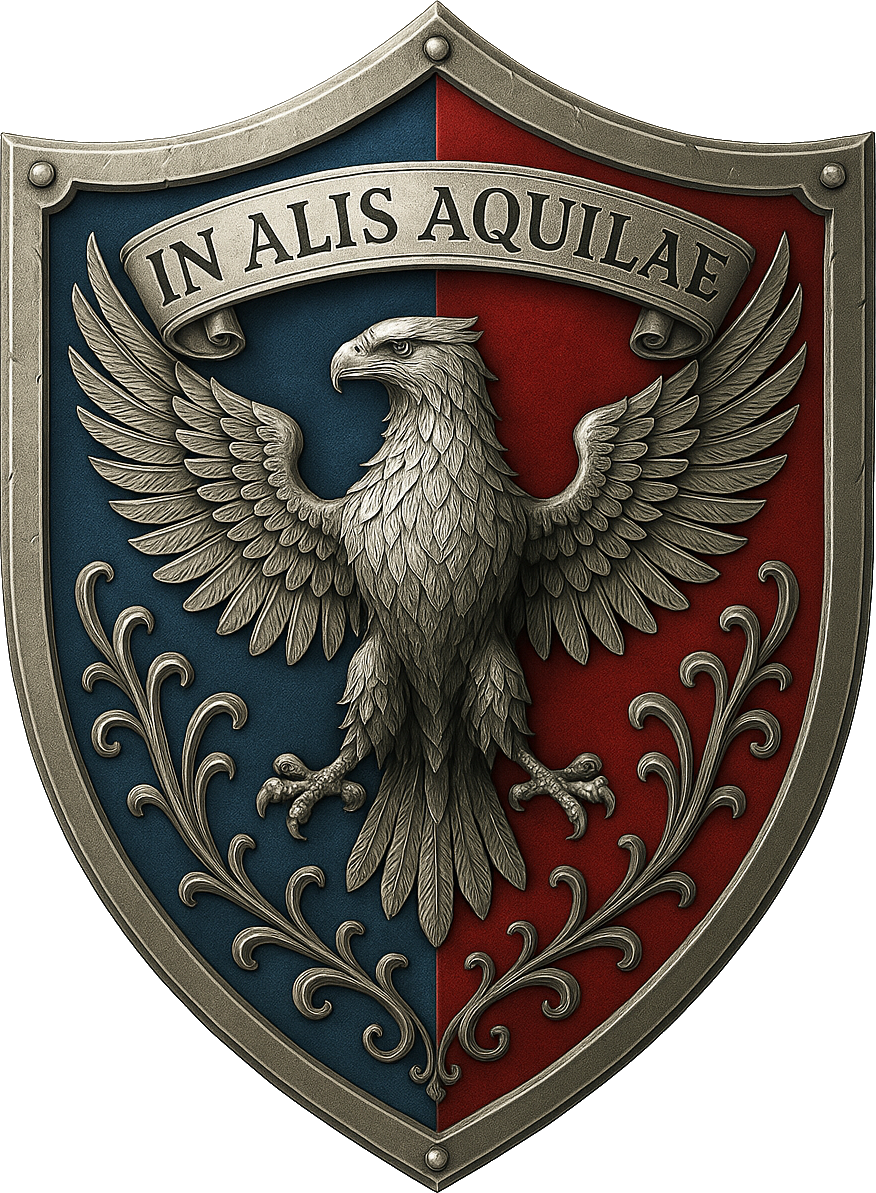
\includegraphics[width=0.1325\textwidth]{Factions/Knights_of_Crail.png}
	\end{tabular}
\end{tabular}
\vspace*{-1.65\fontdimen6\font}\hfill\\{\entryfont breaking enemy ranks on the battlefield, though countless innocents perished. The peace that followed united Crail with Fife under the new Kingdom of Fife, its capital at Dundee. Even now the Order stands apart: sworn to uphold honour and justice, they pledge fealty to the crown but answer only to their Grandmaster.}
\subsubsection*{Eagle Druids of Crail}
\vspace*{-0.7\fontdimen6\font}\hfill\\\begin{tabular}{p{0.3\textwidth}p{0.1325\textwidth}}
	\hspace*{-1.2em}\begin{tabular}[t]{p{0.325\textwidth}}
		{\entryfont The Eagle Druids of Crail are a revered circle tasked with the sacred duty of hatching, nurturing, and bonding with the majestic Great Eagles of Crail. Nestled within the windswept cliffs of Fledgling's Cove, they live in harmony with the colossal raptors, guiding them with\linebreak}
	\end{tabular}
	&
	\vspace*{-2.4em}\begin{tabular}[t]{p{0.1325\textwidth}}
		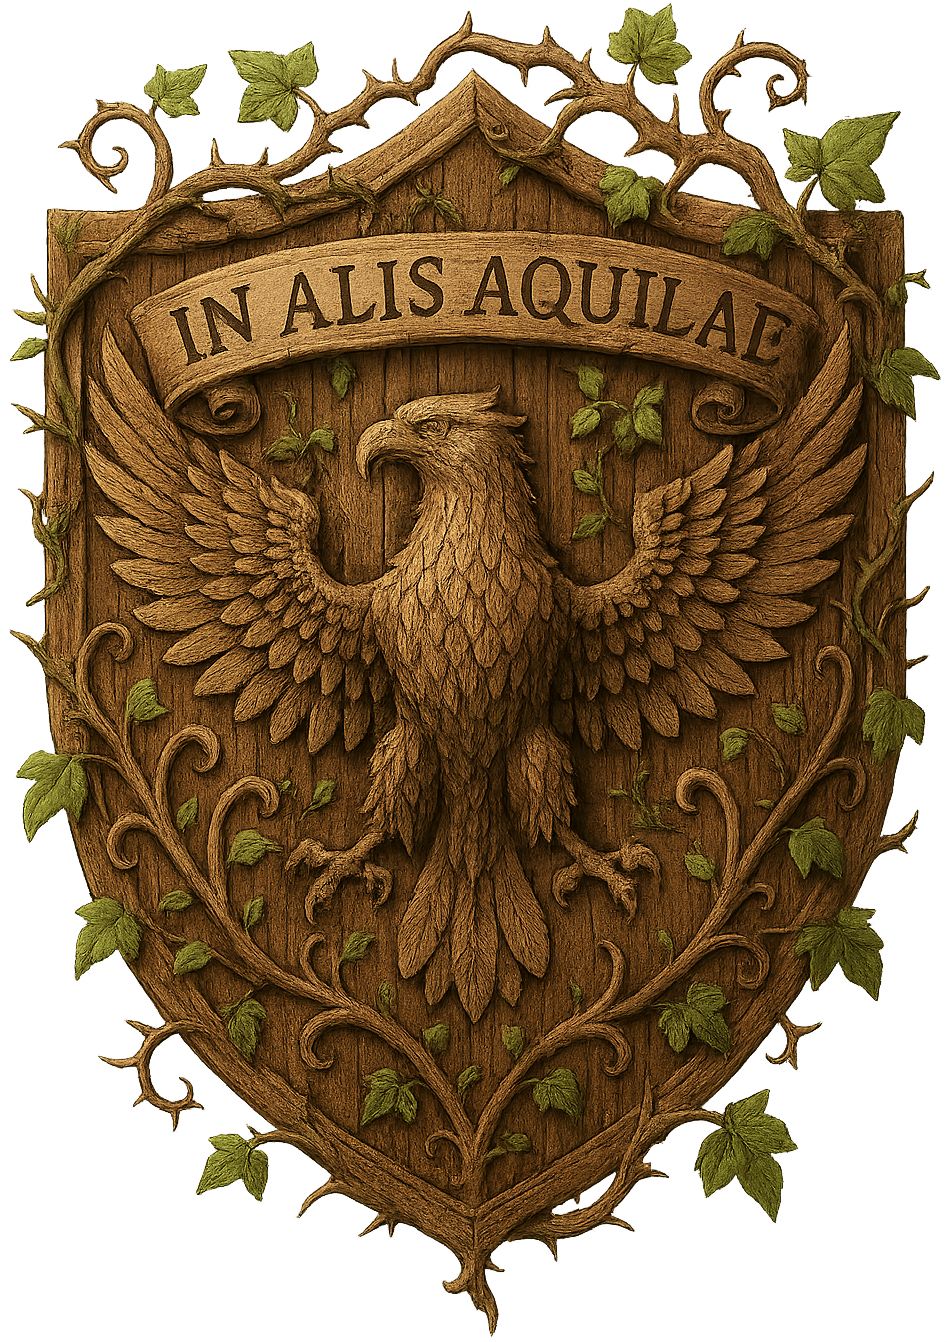
\includegraphics[width=0.1325\textwidth]{Factions/Eagle_Druids_of_Crail.png}
	\end{tabular}
\end{tabular}
\vspace*{-1.65\fontdimen6\font}\hfill\\{\entryfont ancient rites and druidic magic. To be chosen as one of their number is a rare honour, marking one as a guardian of Crail's skies and a spiritual link between the city and its soaring protectors. Their wisdom and prestige echo far beyond the citadel walls, earning them respect throughout the Kingdom of Fife.}
\subsection*{Dwarves of Caledonia}
{\entryfont Two proud dwarven clans have been locked in a generational feud over the truest expression of their people's birthright: is their innate magic best honed at the anvil, weaving runes into living steel, or distilled in bubbling vats, forging power through alchemical art? Each clan jealously guards its traditions and secrets - one honing weapons and armour of unrivaled craftsmanship, the other brewing elixirs and ales that reshape flesh and mind.}
\subsubsection*{Aberdeenshi Dwarves}
\vspace*{-0.7\fontdimen6\font}\hfill\\\begin{tabular}{p{0.3\textwidth}p{0.1325\textwidth}}
	\hspace*{-1.2em}\begin{tabular}[t]{p{0.325\textwidth}}
		{\entryfont Perched in hill-carved holdfasts around Aberdeen, these dwarves weave ancient runes into every ingot. Their forges, built atop converging ley lines, glow with molten magic as master-smiths\linebreak}
	\end{tabular}
	&
	\vspace*{-2.4em}\begin{tabular}[t]{p{0.1325\textwidth}}
		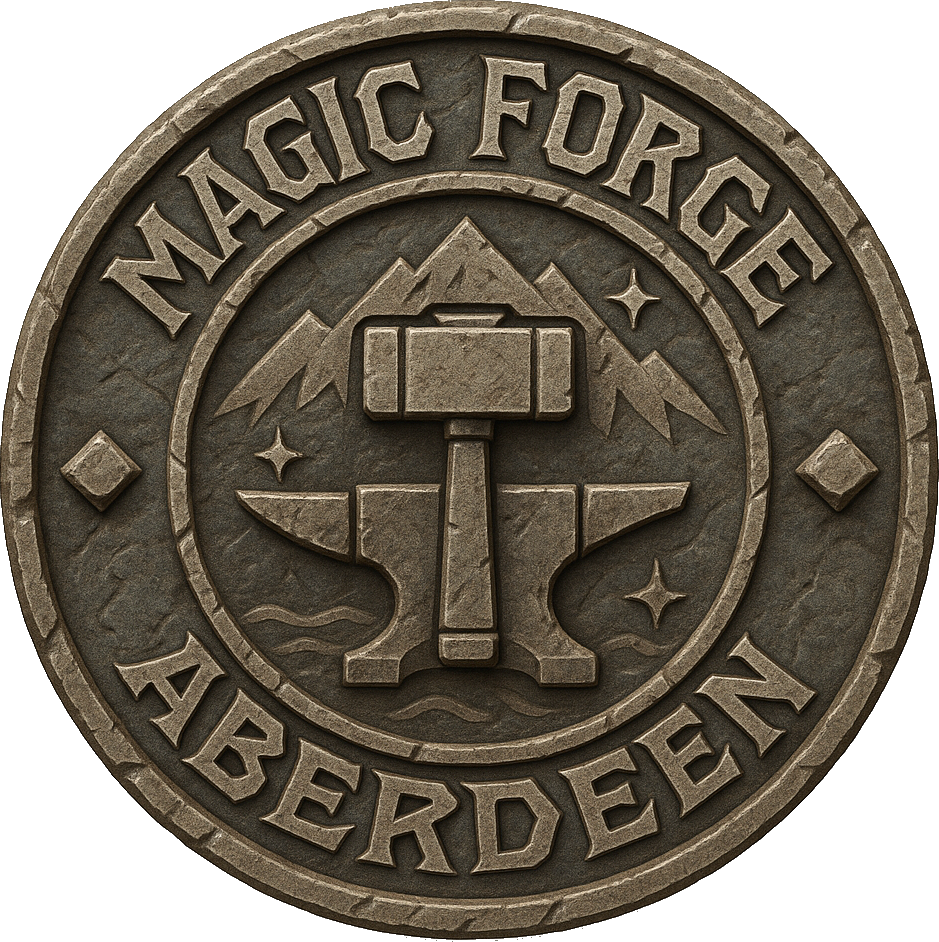
\includegraphics[width=0.1325\textwidth]{Factions/Aberdeenshi_Dwarves.png}
	\end{tabular}
\end{tabular}
\vspace*{-1.65\fontdimen6\font}\hfill\\{\entryfont hammer out blades and plate mail famed for near-living responsiveness. Each weapon whispers with elemental wards - arrows that fly truer, swords that shatter curses, armour that hardens at a touch - earning them renown among knights and mercenaries alike.}
\subsubsection*{Methven Dwarves}
\vspace*{-0.7\fontdimen6\font}\hfill\\\begin{tabular}{p{0.3\textwidth}p{0.1325\textwidth}}
	\hspace*{-1.2em}\begin{tabular}[t]{p{0.325\textwidth}}
		{\entryfont Below the settlement of Methven, the dwarves cultivate subterranean breweries and alchemical labs. In vaulted cellars carved from dragonstone, they blend phosphorescent fungi, enchanted\linebreak}
	\end{tabular}
	&
	\vspace*{-2.4em}\begin{tabular}[t]{p{0.1325\textwidth}}
		
\includegraphics[width=0.1325\textwidth]{Factions/Methven_Dwarves.png}
	\end{tabular}
\end{tabular}
\vspace*{-1.65\fontdimen6\font}\hfill\\{\entryfont waters, and crushed gemstone dust into elixirs and ales of astonishing power. Their draughts can mend shattered bones, sharpen the mind's edge, or unleash berserker strength - each batch a guarded masterpiece. To them, the halflings and humans who stagger from their taverns in awed reverence prove that magic's greatest gift is not tempered steel but the spirit it kindles.}
\subsection*{Elves of Dùn Èideann}
{\entryfont South of the Kingdom of Fife, across the mist-shrouded Firth of Forth, lies the realm of Dùn Èideann - home to a dozen proud elven tribes, each as distinct as the moonlight dancing on its silver towers. Though the deep waters limit traffic to a handful of enchanted ferries and caravans, a steady trickle of goods, lore, and diplomacy flows between the two realms.}
\subsubsection*{Aeloria (High Elves)}
\vspace*{-0.7\fontdimen6\font}\hfill\\\begin{tabular}{p{0.3\textwidth}p{0.1325\textwidth}}
	\hspace*{-1.2em}\begin{tabular}[t]{p{0.325\textwidth}}
		{\entryfont In the vaulted Arcanum Halls of Dùn Èideann, the Aeloria bend raw magic to weave enchantment into steel, wood, and stone. Fluid circles of silver and sapphire shimmer on workbenches as apprentices\linebreak}
	\end{tabular}
	&
	\vspace*{-2.4em}\begin{tabular}[t]{p{0.1325\textwidth}}
		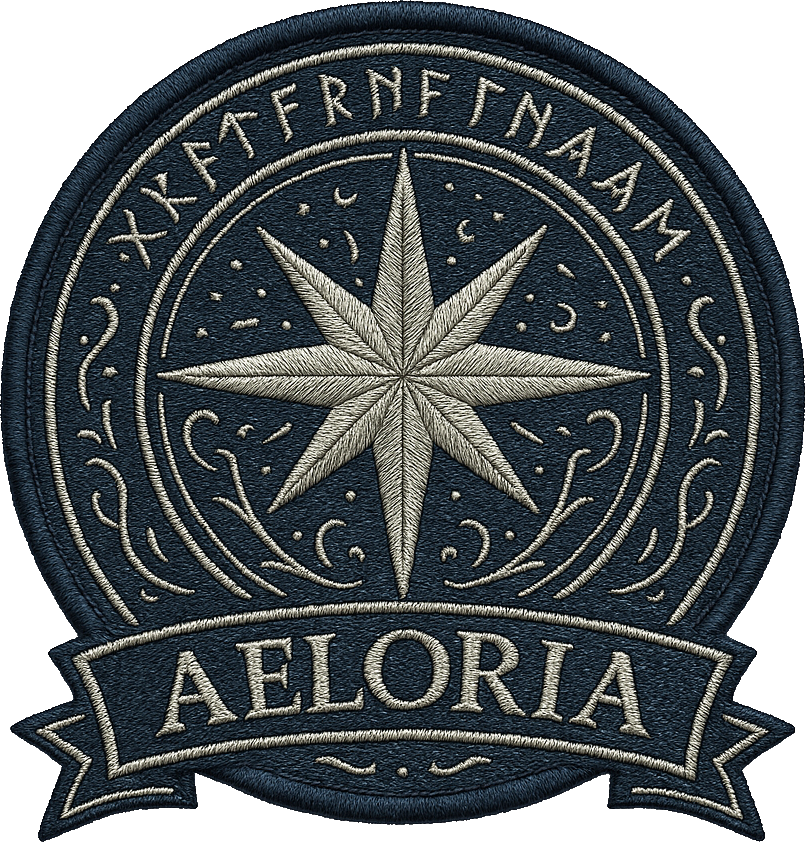
\includegraphics[width=0.1325\textwidth]{Factions/Aeloria.png}
	\end{tabular}
\end{tabular}
\vspace*{-1.65\fontdimen6\font}\hfill\\{\entryfont channel moon-tide energy through crystalline focus orbs, infusing tools with precise enchantments: silent footsteps, flame-touched edges, or strands of shadow-cloak. At the heart of their order stands the Runeheart Sanctum, where senior enchanter convene each solstice to renew the city's protective wards and debate the mysteries of aetheric resonance - ensuring every enchanted object carries a spark of Aelorian brilliance.}
\subsubsection*{Sylvani (Wood Elves)}
\vspace*{-0.7\fontdimen6\font}\hfill\\\begin{tabular}{p{0.3\textwidth}p{0.1325\textwidth}}
	\hspace*{-1.2em}\begin{tabular}[t]{p{0.325\textwidth}}
		{\entryfont Deep within the wooded Pentland Hills of Dùn Èideann's southern groves dwell the Sylvani, a hidden elven tribe whose treetop homes spiral like living sculptures around ancient oaks. By moonlight, vine-woven\linebreak}
	\end{tabular}
	&
	\vspace*{-2.4em}\begin{tabular}[t]{p{0.1325\textwidth}}
		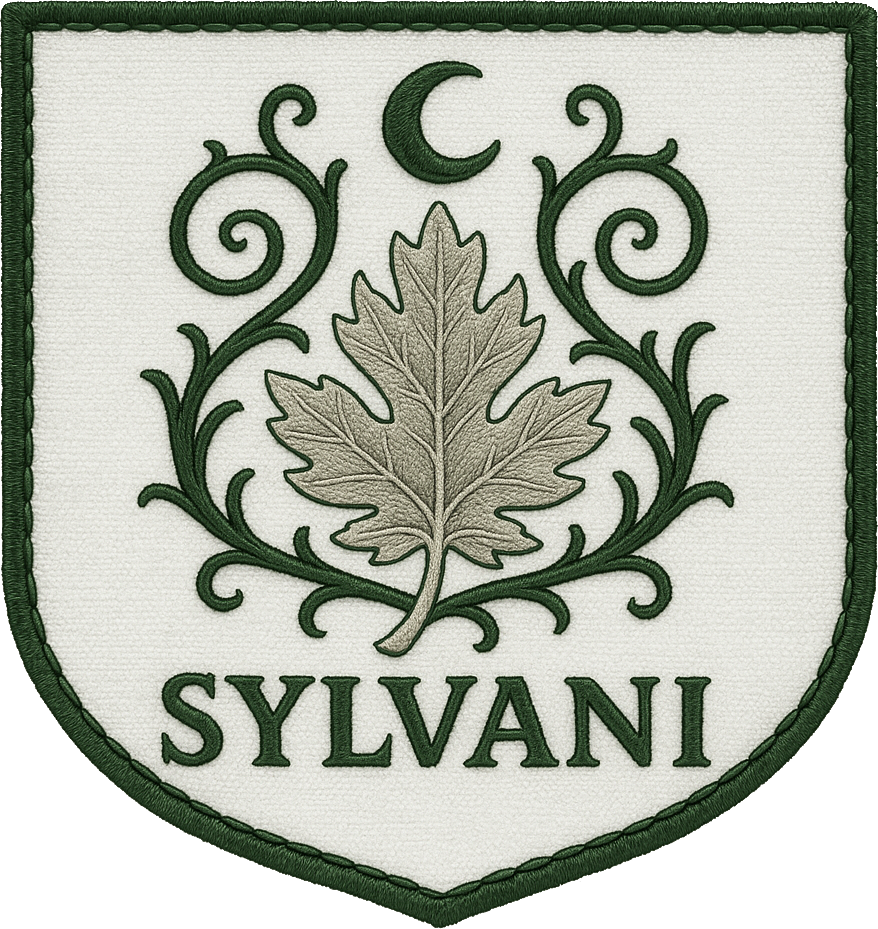
\includegraphics[width=0.1325\textwidth]{Factions/Sylvani.png}
	\end{tabular}
\end{tabular}
\vspace*{-1.65\fontdimen6\font}\hfill\\{\entryfont bridges connect their lantern-lit platforms, where druids known as Leafwardens tend whispering groves and coax sap to heal broken branches. They trade rare healing herbs and bow wood for tools and medicine, though no iron crosses their sacred thresholds. Governed by a moon-lit Council of Bark and Moon, the Sylvani move in silent harmony with the forest's breath - fierce guardians of every leaf and root.}
\subsubsection*{Umbrasil (Drow Elves)}
\vspace*{-0.7\fontdimen6\font}\hfill\\\begin{tabular}{p{0.3\textwidth}p{0.1325\textwidth}}
	\hspace*{-1.2em}\begin{tabular}[t]{p{0.325\textwidth}}
		{\entryfont In the fathomless caverns beneath Dùn Èideann, the Umbrasil first delved only for veins of moonstone, starsteel ore, and aether-quartz - precious crystals prized by the Aeloria. Generations of\linebreak}
	\end{tabular}
	&
	\vspace*{-2.2em}\begin{tabular}[t]{p{0.1325\textwidth}}
		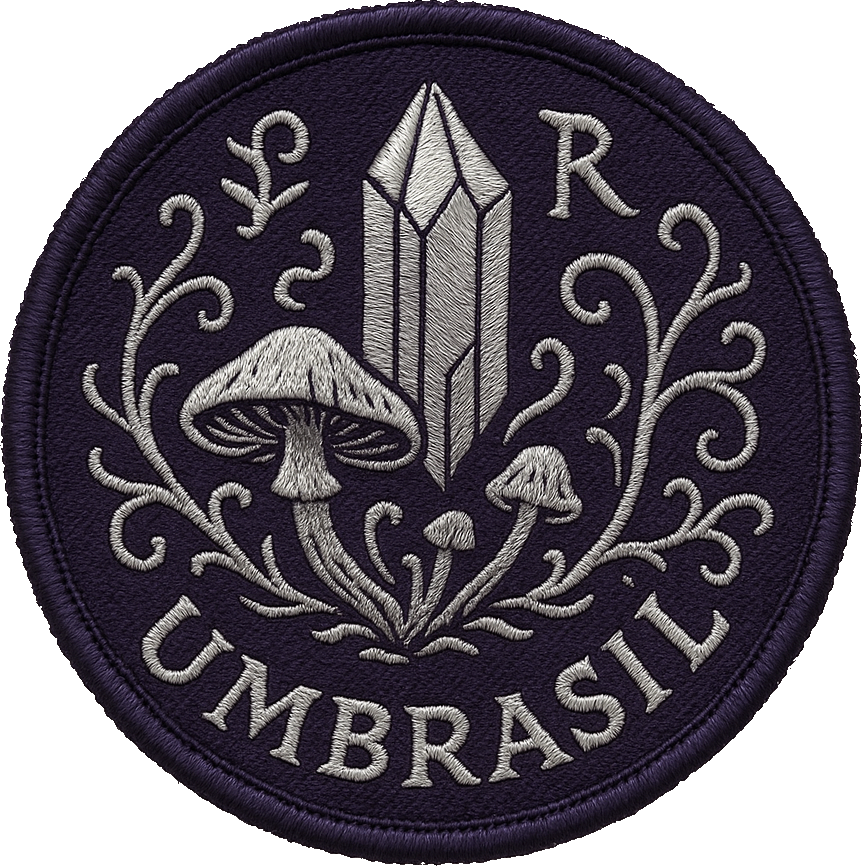
\includegraphics[width=0.1325\textwidth]{Factions/Umbrasil.png}
	\end{tabular}
\end{tabular}
\vspace*{-1.65\fontdimen6\font}\hfill\\{\entryfont tunneling left echoing hollows, until one expedition discovered luminous caps sprouting in these spent veins. Intrigued, their alchemists studied the fungus' phosphorescent spores, unlocking draughts of night-vision, resilience tonics, and dream-weave essences. Thus were born the hidden cultivation caverns - stone-hewn galleries where mycologists coax bio-luminescent crops beside crystal seams. Rare surface-dwellers barter for Umbrasil elixirs but always through high-elf intermediaries, for the Umbrasil trust the light above only as much as it benefits the hidden depths.}
\subsubsection*{Others}
{\entryfont\paragraph*{Mistwalkers} Skiff-borne sea elves who harvest ghostly pearls and shell-silk from hidden reefs, trading these ocean rarities like driftwood carvings and cured sea-urchin spines.}
{\entryfont\paragraph*{Lythari} Elves touched by lycanthropy, they patrol the eastern Firth of Forth at the border of Falkirk and Dunfermlin - amber eyes on the shore to ensure safe passage and ward off threats with bow and fang.}
{\entryfont\paragraph*{Selynari} Elusive moon elves of the North-Western highlands of Caledonia. They flit between mist-cloaked knolls, leaving only crescent glyphs carved in old oaks. Under starlit hush, they perform silent rites of shadow and moonbeam to preserve the hills' hidden magic.}
\subsection*{Lordship of Auchtertool}
\vspace*{-0.3\fontdimen6\font}\hfill\\\begin{tabular}{p{0.3\textwidth}p{0.1325\textwidth}}
	\hspace*{-1.2em}\begin{tabular}[t]{p{0.325\textwidth}}
		{\entryfont The Lordship of Auchtertool is a gleaming forge-city where arcane runes and mechanical gears merge to animate clockwork guardians and towering warforged. Artificers, forge-clerics, and arcane engineers fill its streets with automata familiars, steam-driven\linebreak}
	\end{tabular}
	&
	\vspace*{-2.4em}\begin{tabular}[t]{p{0.1325\textwidth}}
		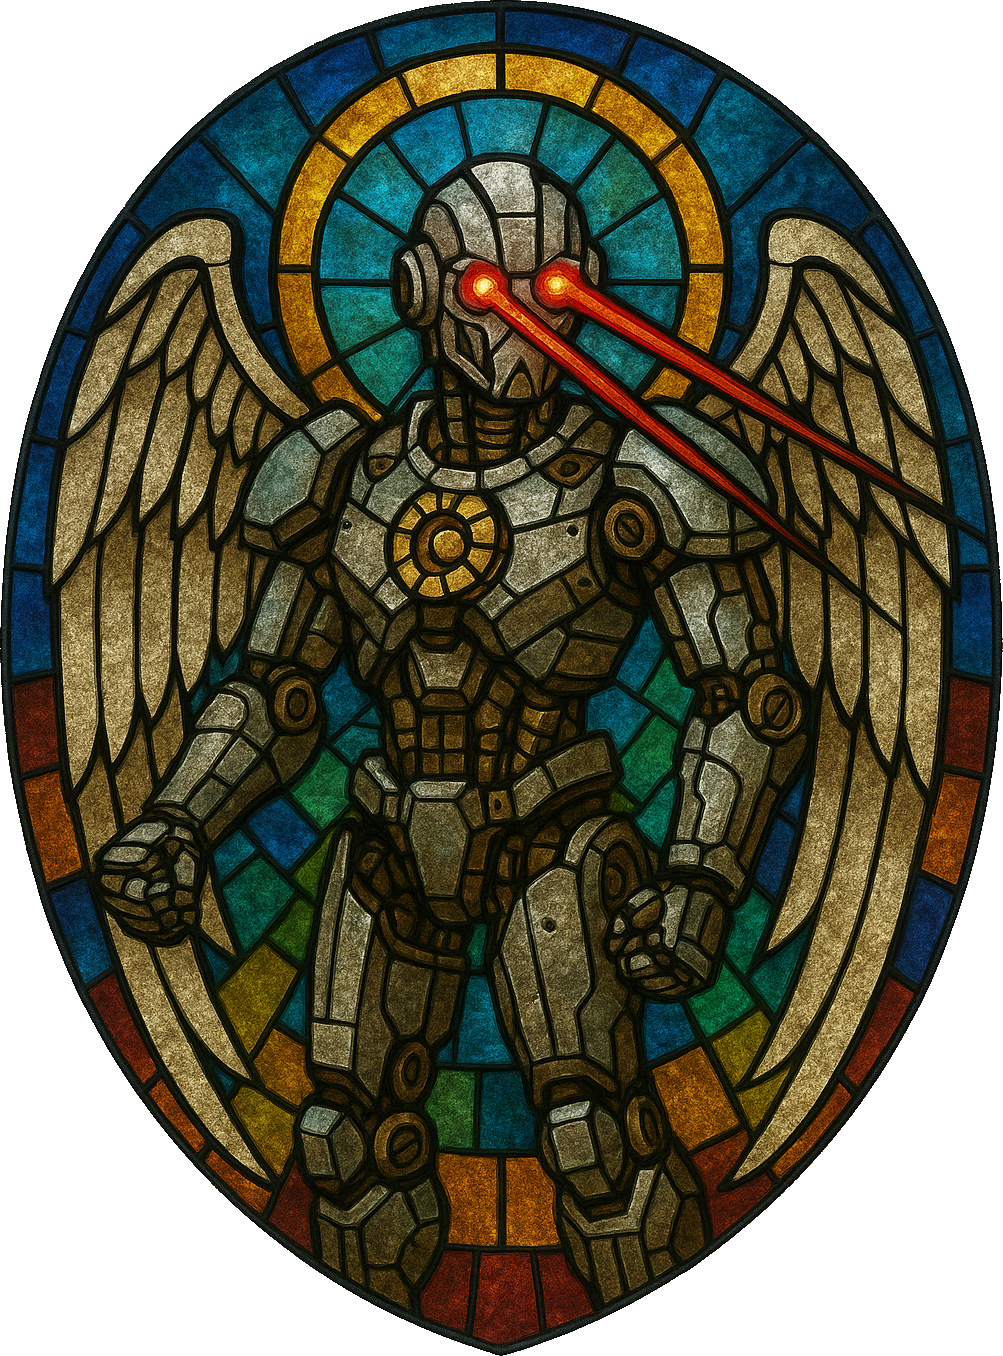
\includegraphics[width=0.1325\textwidth]{Factions/Lordship_of_Auchtertool.png}
	\end{tabular}
\end{tabular}
\vspace*{-1.65\fontdimen6\font}\hfill\\{\entryfont sentinels, and inventions that blur flesh and steel. At its head stands the Mecha-Lord - once a master artificer now encased in enchanted iron - and his heir, the Robot Prince, a sentient bronze construct powered by elemental cores. Together they guide Auchtertool as the kingdom's unrivaled nexus of magical innovation and mechanical marvels.}
\subsection*{Kingdom of Unst}
{\entryfont An island kingdom at Caledonia's northern extreme, Unst is forged in ice and storm, where brutal winters and relentless martial trials - scaling frozen cliffs, sparring on snowbound plains, hurling javelins through blizzards - shape only the toughest into warriors. Under the legendary Hootsman - said to have gargantuous beasts with bare hands - these axe-wielders ride shaggy war-beasts and wear horned helms as they honour feats of raw strength above all else. Feared for their ferocity, they reward those who prove their mettle with unbreakable loyalty.}
\subsection*{Wizards}
\subsubsection*{Courtwizards of Dundee}
\vspace*{-0.7\fontdimen6\font}\hfill\\\begin{tabular}{p{0.3\textwidth}p{0.1325\textwidth}}
	\hspace*{-1.2em}\begin{tabular}[t]{p{0.325\textwidth}}
		{\entryfont Tucked into a cramped turret overlooking the River Tay, the Courtwizards of Dundee bear a grand title belying their modest resources. Under the steady hand of a sole Master Arcanist - rumoured to be\linebreak}
	\end{tabular}
	&
	\vspace*{-2.2em}\begin{tabular}[t]{p{0.1325\textwidth}}
		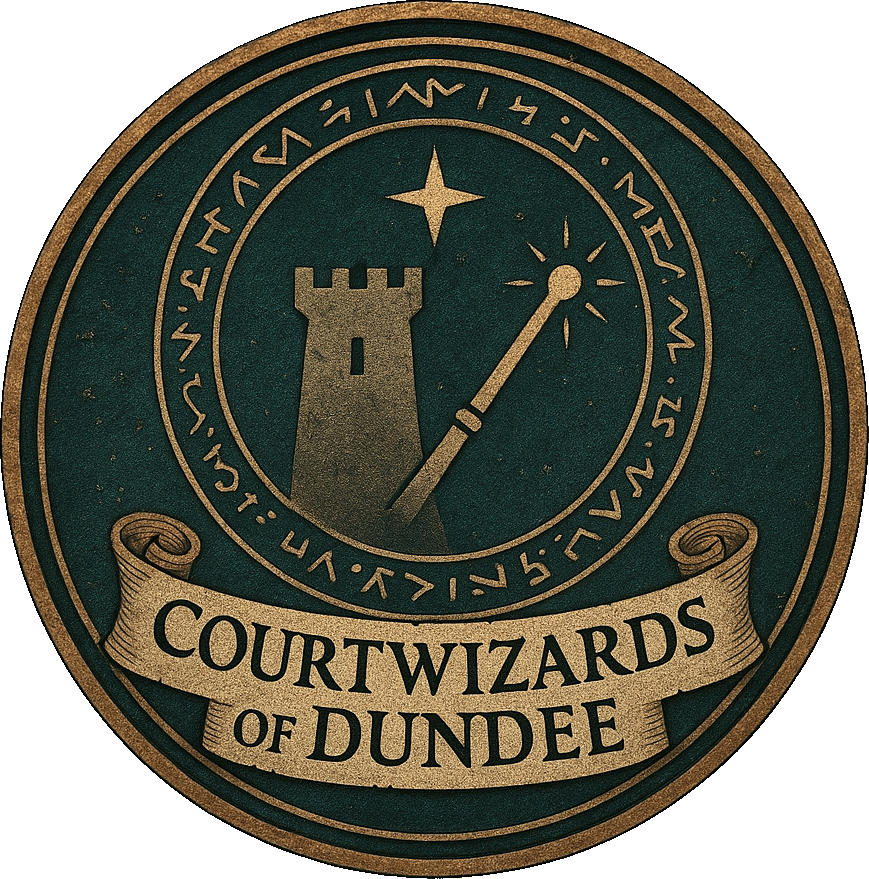
\includegraphics[width=0.1325\textwidth]{Factions/Courtwizards_of_Dundee.png}
	\end{tabular}
\end{tabular}
\vspace*{-1.65\fontdimen6\font}\hfill\\{\entryfont as wise as he is eccentric - a half-dozen apprentices toil over battered grimoires and dented athames. Their workshop is a jumble of cracked crystal balls, tarnished brass astrolabes, and wands salvaged from old duels, yet they manage to weave reliable warding spells around the ducal palace and entertain visiting nobles with small marvels of elemental fire and dancing motes of light. Ambitious but underfunded, they dream of expanding their circle - if only they could persuade the city council to replace cobwebs with coin.}
\subsubsection*{Cairngorm Mountain Wizards}
\vspace*{-0.7\fontdimen6\font}\hfill\\\begin{tabular}{p{0.3\textwidth}p{0.1325\textwidth}}
	\hspace*{-1.2em}\begin{tabular}[t]{p{0.325\textwidth}}
		{\entryfont High amid the snow-shrouded peaks of the Cairngorms lies a near-legendary conclave of wizards whose hidden village seems carved from living granite. Here, beneath ever-churning mists, the wizards practice\linebreak}
	\end{tabular}
	&
	\vspace*{-2.2em}\begin{tabular}[t]{p{0.1325\textwidth}}
		
\includegraphics[width=0.1325\textwidth]{Factions/Cairngorm_Mountain_Wizards.png}
	\end{tabular}
\end{tabular}
\vspace*{-1.65\fontdimen6\font}\hfill\\{\entryfont ancient arts of divination: obsidian runes etched with the world's fate, dream-weaving rituals performed in moonlit amphitheaters, and scrying pools said to reflect tomorrow's sun. Few pilgrims ever breach the winding passes, and of those who do, still fewer return unshaken - bearing cryptic counsel in voices heavy with portent. To meet these mountain mages is to glimpse destiny's edge... if one can decipher their whispered riddles before the wind bears them away.}